
\chapter{Foundations and State of the Art in Intelligent Control for Vehicle-to-Grid Systems}
\vspace*{1cm} % vertical space before the quote

\begin{center}
  \begin{minipage}{0.8\textwidth}
    \begin{displayquote}
      \large\itshape
      ``The green transition is the most ambitious industrial transformation ever. 
      The region of the world that develops clean technologies first will come out on top — 
      and I want it to be Europe.''
    \end{displayquote}
  \end{minipage}
\end{center}

\vspace{0.1cm}

\begin{flushright}
  --- \textsc{Ursula von der Leyen}
\end{flushright}

\section{The V2G Imperative: A Foundation of Europe's Green Transition}
\noindent
Europe finds itself at the confluence of two unprecedented and deeply interlinked transformations reshaping its technological, economic, and societal landscape: the large-scale electrification of transport and a comprehensive restructuring of its energy systems. These parallel transitions involve a radical shift from internal combustion engines to battery electric vehicles and a simultaneous integration of renewable generation, grid modernization, and the deployment of advanced storage and demand-side management solutions.
\noindent
\\
These transformations are not merely aspirational targets but constitute binding legal obligations established under the \textbf{European Green Deal} and the detailed \textbf{"Fit for 55"} legislative package. These frameworks translate climate ambitions into enforceable measures aimed at reducing net greenhouse gas emissions by 55\% by 2030 \cite{european_commission_2021_fit_for_55}. This policy architecture necessitates the rapid phase-out of fossil-fuelled vehicles alongside a dramatic expansion of renewable energy capacity, a goal further reinforced by the revised \textbf{Renewable Energy Directive (RED III)}, as detailed in Figure \ref{fig:RED3}.
 \noindent The figure highlights the significantly increased ambition in RED III, including a higher overall renewable energy target, a more aggressive goal for the transport sector, and stricter requirements for traceability and legal enforceability. This escalation in policy ambition underscores the critical need for flexibility solutions like V2G to manage the grid and integrate higher shares of renewables.
\begin{figure}[H]
    \centering
    \includegraphics[width=0.9\linewidth]{red.png}
    \caption{Comparison of key targets between the Renewable Energy Directive II (RED II, 2018) and the revised RED III (2023).}
    \label{fig:RED3}
\end{figure}

\noindent
Electric Vehicles (EVs) occupy a central position in this transition, simultaneously driving decarbonisation efforts while presenting complex challenges for grid stability. The initial response to mass EV adoption was characterised by concern within the power sector, viewing millions of new EVs as vast, correlated loads threatening to overwhelm distribution networks. This perspective has undergone a fundamental reassessment. EVs are now recognised not as burdens to be managed, but as essential, flexible assets for achieving Europe's energy objectives.
\\
This conceptual shift finds its most concrete expression in \textbf{Vehicle-to-Grid (V2G)} technology, which fundamentally reimagines the role of electric vehicles within the energy system.
\\
\noindent
V2G technology transforms previously passive, unidirectional energy consumers into active, distributed, and intelligent grid resources. The underlying opportunity is substantial: private vehicles spend approximately 96\% of their operational lifetime parked \cite{Englberger2021}, representing an enormous, geographically distributed, and currently underutilised repository of mobile energy storage.
\\
\noindent
The transformative potential of V2G becomes apparent when individual vehicles are coordinated through centrally managed aggregation. While a single EV's contribution is modest, an orchestrated fleet can function as a unified \textbf{Virtual Power Plant (VPP)}. These software-defined power plants aggregate the collective capacity of numerous distributed energy resources, delivering grid services at scales comparable to conventional generation facilities. The rapid response characteristics of contemporary battery inverters, operating at millisecond timescales, enable these aggregated fleets to provide a comprehensive range of critical grid services. This capability is a prerequisite for maintaining stability in grids increasingly dependent on variable wind and solar generation, thereby enabling the technical and economic viability of the EU's ambitious renewable energy targets \cite{Tavakoli2019}.


This \ref{{fig:rl_v2g_ops} diagram illustrates the multifaceted roles an EV fleet
can play, orchestrated by an aggregator using RL. Key operations include gridstabilizing services (frequency control, demand response), economic optimization
(bidding and pricing strategies), and user-centric management (energy storage,
battery health). The objectives range from reducing electricity costs and enhancing
grid flexibility to ensuring data privacy and transaction security, showcasing the
complexity of optimizing V2G operations
\begin{figure}[H]
    \centering
    \includegraphics[width=0.9\linewidth]{Reinforcement_learning_V2G_operations.png}
    \caption{Reinforcement learning (RL) applications in V2G from the perspective of participating entities.}
    \label{fig:rl_v2g_ops}
\end{figure}

\noindent
The grid services enabled by V2G technology, many of which are illustrated in Figure \ref{fig:rl_v2g_ops}, form the technical foundation for the smart, resilient, and decarbonised electricity system required for Europe's energy future:
\\
\noindent
\textbf{Frequency Regulation:} Grid stability depends on maintaining a precise equilibrium between electricity supply and demand, manifested as a stable grid frequency (50 Hz in Europe). Deviations signal imbalances that can trigger cascading failures. V2G fleets, with their rapid-response inverters, can participate in ancillary service markets like Frequency Containment Reserve (FCR) and automatic Frequency Restoration Reserve (aFRR), injecting or absorbing power within seconds to counteract deviations and prevent blackouts \cite{alfaverh2022optima, white2011vehicle}.
\\
\noindent 
\textbf{Demand Response and Peak Shaving:} By intelligently shifting charging to off-peak periods and strategically discharging during peak demand, V2G systems flatten daily load profiles. This directly mitigates the "duck curve" phenomenon (Figure \ref{fig:duck_curve}) associated with high solar penetration. Such load management reduces reliance on expensive, carbon-intensive "peaker" plants and can defer or eliminate costly grid infrastructure upgrades \cite{orfanoudakis2024ev2gym, sadeghi2022deep}.\noindent
Net load is the total electricity demand minus variable renewable energy generation. The deepening "belly" of the duck during midday reflects overgeneration from solar power, while the steep "neck" in the evening represents a rapid increase in demand as solar generation fades. This steep ramp poses a significant challenge for grid operators. V2G helps mitigate this by absorbing excess energy during the day (charging) and discharging it during the evening ramp to "flatten the curve".\cite{Bisetto_Francesca}

\begin{figure}[H]
    \centering
    \includegraphics[width=0.8\linewidth]{duck.png}
    \caption{The "Duck Curve" illustrating the evolution of net load on the California grid.}
    \label{fig:duck_curve}
\end{figure}

\noindent
\textbf{Renewable Energy Integration:} The most strategically significant contribution of V2G is addressing renewable energy intermittency. V2G fleets act as large-scale energy buffers, absorbing excess solar and wind generation that would otherwise be curtailed. This stored energy is then released during periods of low generation. This mechanism directly increases the utilisation of renewable resources, supporting the integration objectives of RED III and enhancing overall system efficiency.
\\
\noindent
\textbf{Economic and Market Optimization:} Beyond grid stability, V2G enables sophisticated market participation. As shown in Figure \ref{fig:rl_v2g_ops}, aggregators can deploy intelligent bidding and pricing strategies. Reinforcement learning algorithms can learn optimal policies for participating in day-ahead and intraday energy markets, maximizing revenue for both the aggregator and EV owners by capitalizing on price volatility.
\\
\noindent
\textbf{User-Centric Management and Security:} For V2G to succeed, it must align with user needs and address concerns. This includes optimizing charging and discharging cycles to minimize \textbf{battery degradation}, thus preserving vehicle lifespan. Furthermore, as V2G involves financial transactions and data exchange, robust \textbf{cyber security} is paramount to protect user privacy and ensure transaction security, another key domain for intelligent management systems.
\\
\noindent
This vision is being actively incorporated into European legal frameworks. The transformative \textbf{Alternative Fuels Infrastructure Regulation (AFIR, EU 2023/1804)} now mandates that new public charging infrastructure incorporate smart and bidirectional capabilities. This is supported by technical standards like \textbf{ISO 15118-20}, which specifies protocols for a "Vehicle-to-Grid Communication Interface" (V2GCI). With mandatory implementation scheduled for 2027, the necessary infrastructure is being systematically established, supported by pilot initiatives like the \textbf{'SCALE'} and \textbf{'V2G Balearic Islands'} projects.
\\
\noindent
Despite this progress, substantial obstacles to widespread V2G deployment persist:

\begin{itemize}
    \item \textbf{Market and Economic Barriers:} A coherent, pan-European framework for compensating EV owners for grid services is still undeveloped. Accessing existing value streams is complex, and issues like the \textbf{"double taxation"} of electricity—taxing energy during both charging and discharging—create significant economic disincentives.
    
    \item \textbf{Regulatory and Grid Access Challenges:} The qualification of EV fleets as flexibility resources varies across national markets. Standardised procedures for grid interconnection, aggregator certification, and secure data exchange are needed to reduce fragmentation and simplify commercial deployment.
    
    \item \textbf{Technical and Consumer Adoption Barriers:} Consumer concerns regarding accelerated \textbf{battery degradation} and its impact on vehicle warranties are primary obstacles. Furthermore, much of the current EV and charging infrastructure lacks bidirectional capability, though this is changing with new vehicle platforms and standards.
\end{itemize}
\noindent
The fundamental challenge addressed by this thesis extends beyond simply enabling V2G technology to encompass its \textit{intelligent orchestration}. This requires developing control strategies sophisticated enough to operate within emerging regulatory frameworks, navigate economic uncertainties, accommodate diverse user preferences, and overcome technical constraints. The objective is to unlock the substantial potential of EVs as fundamental components of Europe's energy transition while ensuring system reliability, economic viability, and user acceptance.
%%%%%%%%%%%%%%%%%%%%%%%%%%%%%%
%%%%%%%%%%%%%%%%%%%%%%%%%%%%%%

%%%%%%%%%%%%%%%%%%%%%%%%%%%%%%

%%%%%%%%%%%%%%%%%%%%%%%%%%%%%%


%%%%%%%%%%%%%%%%%%%%%%%%%%%%%%

%%%%%%%%%%%%%%%%%%%%%%%%%%%%%%
\section{The Optimizer's Trilemma: Navigating a Stochastic World}
While the potential of V2G technology is substantial, the management of distributed vehicular assets presents a complex control challenge. Economic viability drives aggregator decisions, yet a narrow focus on profitability alone proves insufficient for sustainable operations. Effective V2G management requires balancing three competing objectives that frequently conflict with one another. This challenge can be framed as the "V2G Optimizer's Trilemma": the concurrent pursuit of \textbf{economic profitability}, preservation of \textbf{battery longevity}, and maintenance of \textbf{user convenience}.
\noindent
Rather than representing a straightforward, static trade-off, this constitutes a dynamic, multi-objective optimisation challenge characterised by \textbf{stochasticity} and \textbf{uncertainty} arising from multiple, interconnected sources \cite{wang2022multi}:
\\
    \noindent
    \textbf{Market Volatility:} Wholesale electricity prices exhibit significant variability driven by unpredictable supply variations (such as sudden reductions in wind generation capacity) and demand fluctuations (including heat-driven increases in cooling demand). Effective control systems must respond to these price signals dynamically and in real-time.
 \\
    \noindent   
\textbf{Renewable Intermittency:} Co-located solar and wind generation exhibit inherently variable output patterns with limited predictability. Controllers must coordinate EV fleet operations to capture available generation during surplus periods without compromising other operational objectives.
    \\
    \noindent
  \textbf{Human Behaviour:} Perhaps the most challenging uncertainty source involves EV owner patterns. Arrival times, departure schedules, and required state of charge (SoC) at departure lack deterministic characteristics. Emergency departures or unexpected schedule changes represent hard, non-negotiable constraints that intelligent systems must accommodate to preserve user trust and satisfaction.

\noindent
This dynamic, uncertain, and multifaceted operational environment renders static, rule-based control approaches (such as "charge when price falls below threshold X, discharge when exceeding threshold Y") inadequate and brittle. More sophisticated and adaptive methodologies are required,approaches capable of learning from operational experience and making optimal decisions under conditions of significant uncertainty. Reinforcement Learning excels in precisely this domain, providing a framework for developing control policies that demonstrate robustness, adaptability, and scalability.




%%%%%%%%%%%%%%%%%%%%%%%
\subsection{Sources for Energy Price Data}

Access to reliable, real-time, and historical market data remains crucial for both control agent training in simulation environments and real-world deployment. Key public sources for European market data include:
\\
\noindent
 \textbf{ENTSO-E Transparency Platform:} The European Network of Transmission System Operators for Electricity maintains a mandatory, open-access platform serving as a comprehensive repository of pan-European electricity market data. This includes harmonised day-ahead prices, load forecasts, and generation data, serving as the primary source for academic research through both web portal access and free RESTful API services.
    \\
\noindent
    \textbf{National Transmission System Operators (TSOs):} Many national TSOs (including Terna in Italy, National Grid in the UK, and RTE in France) publish detailed market data covering real-time frequency and imbalance prices for their respective jurisdictions.
    \\
\noindent
     \textbf{Power Exchanges:} Exchanges such as \textbf{EPEX SPOT} and \textbf{Nord Pool} constitute actual trading venues. While they represent direct price data sources, comprehensive real-time access typically requires commercial subscription services.


\subsection{Buying vs. Selling: The Critical Retail-Wholesale Spread}

A critical yet frequently overlooked aspect of V2G economics involves the distinction between EV owner charging costs and aggregator grid sales revenue.

\begin{itemize}
    \item \textbf{Selling Price (V2G Revenue):} When EVs provide energy to the grid, revenue calculation bases on \textbf{wholesale prices} (such as day-ahead spot prices). These prices reflect pure marginal energy costs at specific times.
    
    \item \textbf{Buying Price (Charging Cost):} End consumer EV charging costs reflect \textbf{retail prices}, significantly exceeding wholesale prices due to numerous non-energy components, termed "non-commodity costs":
    \begin{itemize}
        \item Base wholesale energy costs
        \item \textbf{Grid Tariffs:} Charges for high-voltage transmission and low-voltage distribution network usage
        \item \textbf{Taxes and Levies:} National or regional taxation including VAT and environmental levies applied to electricity consumption
        \item \textbf{Supplier Margin:} Retail energy provider profit margins
    \end{itemize}
\end{itemize}
\noindent
This substantial gap between retail purchasing prices and wholesale selling prices constitutes the "retail-wholesale spread," creating the primary opportunity for profitable energy arbitrage. Successful control strategies must account for these price differentials to enable economically rational decision-making.

\section{Modelling the V2G Ecosystem}
\label{sec:ev_and_scenario}

Before examining control algorithms, establishing clear, high-fidelity models of system core components becomes essential: the electric vehicle as a controllable cyber-physical asset, and the operational environment or "scenario." The interaction between these elements defines V2G optimisation task boundaries and objectives.

\subsection{The Grid-Interactive EV as a Controllable Asset}


\noindent
From a power grid perspective, electric vehicles represent sophisticated mobile energy storage devices. For V2G applications, EVs can be characterised through several key state variables and parameters:
\\
\noindent
    \textbf{The Battery:} The core grid asset component, defined by \textbf{nominal energy capacity} (in kWh), current \textbf{State of Charge (SoC)}, and \textbf{State of Health (SoH)} representing degradation over time. Operation is constrained by \textbf{power limits} (in kW) dictating maximum charge or discharge rates, and charging/discharging \textbf{efficiencies} accounting for energy losses.
    \\
    \noindent
    \textbf{The On-Board Charger (OBC):} For AC charging applications, the OBC converts grid alternating current to battery direct current. Power rating often constitutes the primary bottleneck for both charging and V2G power output.
    \\
\noindent    
  \textbf{Communication Interface:} V2G participation requires vehicle-charging station (EVSE) communication capabilities. This is governed by standards including \textbf{ISO 15118} and protocols such as the \textbf{Open Charge Point Protocol (OCPP)}, enabling secure information exchange required for smart and bidirectional power flow operations.
\\
\noindent
Combined with vehicle availability patterns—arrival and departure times plus user energy requirements,these characteristics transform EVs from simple loads into fully dispatchable grid resources.

%%%%%%%%%%%%%%%%%%%%%%%%%%%%%%%%%%%%%
%%%%%%%%%%%%%%%%%%%%%%%%%%%%%%%%%%%%%%%%
%%%%%%%%%%%%%%%%%%%%%%%%\section{A New Paradigm for Control: Reinforcement Learning}

\section{A New Paradigm for Control: Reinforcement Learning - Based on the work of Sutton \& Barto}



\begin{center}
    \begin{minipage}{0.8\textwidth}
        \large\itshape
        ``Reinforcement learning is learning what to do---how to map situations to actions---so as to maximize a numerical reward signal.''
    \end{minipage}
\end{center}

\vspace{0.1cm}

\begin{flushright}
--- Richard S. Sutton \& Andrew G. Barto, \textit{Reinforcement Learning: An Introduction} (2018) \cite{Sutton2018}
\end{flushright}

\noindent
To address the complexities of uncertainty, multi-objective trade-offs, and dynamic systems, this work employs Reinforcement Learning (RL), a machine learning paradigm that learns optimal sequential decision-making policies through trial-and-error interaction with an environment. Unlike traditional optimal control methods, which depend on an explicit and accurate model of the environment's dynamics, RL agents learn directly from the outcomes of their actions. This model-free approach provides significant robustness in the face of uncertainty and unmodeled dynamics.

\section{The Reinforcement Learning Problem}
The problem of reinforcement learning is formalized as the interaction between a learning \textbf{agent} and its \textbf{environment}. This interaction unfolds over a sequence of discrete time steps, $t = 0, 1, 2, \dots$.

\subsection{The Agent-Environment Interface}
At each time step $t$, the agent receives a representation of the environment's \textbf{state}, $S_t \in \mathcal{S}$, and on that basis selects an \textbf{action}, $A_t \in \mathcal{A}(S_t)$. One time step later, as a consequence of its action, the agent receives a numerical \textbf{reward}, $R_{t+1} \in \mathcal{R}$, and finds itself in a new state, $S_{t+1}$. This interaction loop forms the foundational framework of the RL problem.

\begin{figure}[H]
    \centering
    % Placeholder for a standard RL interaction diagram
    \includegraphics[width=0.8\linewidth]{RL.png}
    \caption{The agent-environment interaction loop in reinforcement learning \cite{Sutton2018}.}
    \label{fig:rl_loop}
\end{figure}

\subsection{Goals, Rewards, and Returns}
The agent's objective is formalized by the \textbf{reward hypothesis}: that all goals and purposes can be framed as the maximization of the expected cumulative reward. The agent's goal is not to maximize the immediate reward, $R_{t+1}$, but the cumulative reward in the long run. This cumulative reward is known as the \textbf{return}, denoted $G_t$.
\\
\noindent
For \textit{episodic tasks} that terminate, the return is the finite sum of future rewards. For \textit{continuing tasks} that do not terminate, the return is defined as the discounted sum of future rewards:
\begin{equation}
    G_t \doteq \sum_{k=0}^{\infty} \gamma^k R_{t+k+1}
\end{equation}
where $\gamma \in [0, 1)$ is the \textbf{discount factor}. It determines the present value of future rewards, ensuring the infinite sum is finite and balancing immediate gratification against long-term gains. A value of $\gamma=0$ results in a myopic agent concerned only with maximizing immediate rewards.

\section{The Language of Learning: Markov Decision Processes}

The mathematical foundation of Reinforcement Learning (RL) is the \textbf{Markov Decision Process (MDP)}. An MDP provides a formal framework for modeling decision-making in stochastic environments where outcomes are partly random and partly under the control of a decision-maker.
\\
\noindent
An MDP is formally defined as a tuple \( \langle S, A, P, R \rangle \), where:
\begin{itemize}
    \item \(S\) is a finite set of states.
    \item \(A\) is a finite set of actions.
    \item \(P\) is the state transition probability function, \(P(s'|s, a)\), which represents the probability of transitioning to state \(s'\) from state \(s\) after taking action \(a\).
    \item \(R\) is the reward function, \(R(s, a, s')\), which is the immediate reward received after transitioning from state \(s\) to state \(s'\) as a result of action \(a\).
\end{itemize}
\noindent
A key assumption in an MDP is that the environment is fully observable, meaning the agent knows its current state with certainty. However, in many real-world scenarios, the agent may not have complete information about its state. This is where the \textbf{Partially Observable Markov Decision Process (POMDP)} comes into play.
\\
\noindent
A POMDP extends the MDP framework to situations where the agent's observations of the environment are incomplete or noisy. A POMDP is represented by a tuple \( \langle S, A, P, R, \Omega, O \rangle \), which includes all the elements of an MDP plus:
\begin{itemize}
    \item \(\Omega\) is a finite set of observations the agent can receive from the environment.
    \item \(O\) is the observation probability function, \(O(o|s', a)\), which is the probability of observing \(o\) after transitioning to state \(s'\) having taken action \(a\).
\end{itemize}
\begin{figure}[H]
    \centering
   
    \includegraphics[width=0.8\linewidth]{MDP.png}
    \caption{Differences between  POMDP and MDP  \cite{sadeghi2022deep}.}
    \label{fig:mdp}
\end{figure}
\noindent
The fundamental difference between an MDP and a POMDP lies in the agent's perception of the environment's state. In an MDP, the agent directly observes the state \(s\). In a POMDP, the agent receives an observation \(o\) and must infer a belief, which is a probability distribution over the possible states, to make a decision. As discussed in Sadeghi's work, this partial observability in POMDPs introduces a significant layer of complexity because the agent must act based on a belief state rather than a certain state.\cite{sadeghi2022deep}
\\
\noindent
In our current discussion, we will focus on the MDP framework, assuming that the state of the environment is fully observable to the agent.
\subsection{The Markov Property}
The future is independent of the past given the present. A state signal $S_t$ is said to have the \textbf{Markov Property} if the environment's response at time $t+1$ depends only on the state and action at time $t$. The probability of transitioning to state $s'$ and receiving reward $r$ is independent of all previous states and actions:
\begin{equation}
    p(s', r | s, a) \doteq \Pr\{S_{t+1}=s', R_{t+1}=r | S_t=s, A_t=a\}
\end{equation}
This property is fundamental as it allows decisions to be made based solely on the current state, without needing the complete history of interaction.

\subsection{Policies and Value Functions}
The agent's learning objective is to find a good \textbf{policy}, $\pi(a|s)$, which is a mapping from states to probabilities of selecting each possible action. The goodness of a policy is assessed by its \textbf{value functions}.
\begin{itemize}
    \item The \textbf{state-value function}, $v_\pi(s)$, is the expected return starting from state $s$ and following policy $\pi$ thereafter:
    \begin{equation}
        v_\pi(s) \doteq \mathbb{E}_\pi [G_t | S_t=s]
    \end{equation}
    \item The \textbf{action-value function}, $q_\pi(s, a)$, is the expected return starting from state $s$, taking action $a$, and thereafter following policy $\pi$:
    \begin{equation}
        q_\pi(s, a) \doteq \mathbb{E}_\pi [G_t | S_t=s, A_t=a]
    \end{equation}
\end{itemize}

\section{The Bellman Equations}
The Bellman equations provide a recursive decomposition that is foundational to solving MDPs. They express the value of a state in terms of the values of its successor states.

\subsection{The Bellman Expectation Equation}
For a given policy $\pi$, the state-value function must satisfy a self-consistency condition. The value of a state equals the expected immediate reward plus the discounted expected value of the next state:
\begin{equation}
    v_\pi(s) = \sum_a \pi(a|s) \sum_{s', r} p(s', r | s, a) [r + \gamma v_\pi(s')]
\end{equation}
This is the \textbf{Bellman expectation equation} for $v_\pi$. It forms the basis for policy evaluation algorithms.

\subsection{The Bellman Optimality Equation}
The ultimate goal is to find an \textbf{optimal policy}, $\pi_*$, which is a policy that achieves a higher or equal expected return than all other policies from all states. All optimal policies share the same optimal value functions, $v_*(s)$ and $q_*(s, a)$. The optimal value function for a state is the maximum expected return achievable from that state:
\begin{equation}
    v_*(s) = \max_a \mathbb{E}[R_{t+1} + \gamma v_*(S_{t+1}) | S_t=s, A_t=a] = \max_a \sum_{s', r} p(s', r | s, a) [r + \gamma v_*(s')]
\end{equation}
This is the \textbf{Bellman optimality equation}. Solving it means finding the optimal policy.

\subsection{Generalized Policy Iteration (GPI)}
Most RL algorithms can be understood within the framework of \textbf{Generalized Policy Iteration (GPI)}, as described in Chapter 4 of \cite{Sutton2018}. GPI refers to the general idea of letting two interacting processes, policy evaluation and policy improvement, work towards a common optimal solution.

\begin{itemize}
    \item \textbf{Policy Evaluation}: Given a policy $\pi$, compute its value function $v_\pi$. This step aims to make the value function consistent with the current policy.
    \item \textbf{Policy Improvement}: Given a value function $v$, improve the policy by making it greedy with respect to $v$. For a given state $s$, the new policy will select the action $a$ that maximizes $q_\pi(s, a)$.
\end{itemize}
\noindent
These two processes compete in the short term (improving the policy makes the value function inaccurate) but cooperate in the long term to converge to the optimal policy and optimal value function. \textbf{Dynamic Programming (DP)} methods like policy iteration and value iteration are classic examples of GPI, assuming a perfect model of the environment.

\section{Learning from Experience: MC and TD Methods}
When a model of the environment is not available, we must learn from sampled experience. Chapters 5 and 6 of \cite{Sutton2018} introduce two primary model-free approaches.

\subsection{Monte Carlo (MC) Methods}
MC methods learn value functions by averaging the returns from sample episodes.
\begin{itemize}
    \item \textbf{Principle}: An update to $V(S_t)$ is made only at the end of an episode.
    \item \textbf{Update Target}: The target for the update is the actual, complete return $G_t$.
    \item \textbf{Update Rule} (Constant-$\alpha$): $V(S_t) \leftarrow V(S_t) + \alpha [G_t - V(S_t)]$
    \item \textbf{Properties}: MC methods are unbiased but can have high variance and are only applicable to episodic tasks. They do not \textit{bootstrap} \footnote{It means that MC updates only from complete sampled returns.}.
\end{itemize}

\subsection{Temporal-Difference (TD) Learning}
TD learning is a central and novel idea in RL, combining ideas from both MC and DP.
\begin{itemize}
    \item \textbf{Principle}: TD methods update the value estimate for a state based on the observed reward and the estimated value of the successor state. They learn from incomplete episodes.
    \item \textbf{Update Target}: The target is an estimate of the return, called the TD Target: $R_{t+1} + \gamma V(S_{t+1})$.
    \item \textbf{Update Rule} (TD(0)): $V(S_t) \leftarrow V(S_t) + \alpha [R_{t+1} + \gamma V(S_{t+1}) - V(S_t)]$
    \item \textbf{Properties}: TD methods \textit{bootstrap}:they update a guess from a guess. This introduces bias but often leads to lower variance and faster learning. They are naturally implemented in an online, fully incremental fashion.
\end{itemize}

\section{Actor-Critic Architectures}
The \textbf{Actor-Critic} architecture provides a powerful and widely adopted method for solving RL problems, particularly in continuous action spaces. It explicitly represents both the policy and the value function using two distinct function approximators (e.g., neural networks).

\begin{itemize}
    \item \textbf{The Critic}: Learns a value function (e.g., $v_\pi(s)$ or $q_\pi(s, a)$). Its role is to evaluate the actor's decisions by computing the TD error:
    \begin{equation}
        \delta_t = R_{t+1} + \gamma V(S_{t+1}) - V(S_t)
    \end{equation}
    \item \textbf{The Actor}: Represents the policy, $\pi_\theta(a|s)$, parameterized by $\theta$. It receives the current state as input and outputs an action. It uses the TD error from the critic as a learning signal to update its parameters via policy gradient methods, improving its strategy over time.
\end{itemize}
\noindent
This separation of concerns allows for direct policy optimization in continuous or large action spaces while leveraging the stable learning dynamics of TD-based value estimation.
% ===================================================================
% REWARD SHAPING SECTION
% ===================================================================
 \section{Reward Engineering: Shaping Agent Behavior}
\label{sec:reward_shaping}

The design of an effective reward function is arguably the most critical aspect of any Reinforcement Learning (RL) system.
It serves as the primary communication channel through which designers convey desired behaviors and objectives to a learning agent. 
A poorly designed reward function can lead to agents learning unintended, suboptimal, or even harmful behaviors,despite successfully maximizing their assigned objective.
Consequently, reward engineering has emerged as a fundamental and increasingly sophisticated discipline within modern RL,
proving indispensable for the successful application of algorithms in complex, real-world scenarios \footcite{ibrahim2024comprehensive}.
\noindent
The Vehicle-to-Grid (V2G) challenge, with its inherent multi-objective nature,encompassing profit maximization, assurance of user satisfaction, preservation of battery health, and maintenance of grid stability—presents particularly stringent demands on reward function design.
\noindent
This section investigates several advanced techniques for effectively guiding agent learning in such intricate environments.

\subsection{Potential-Based Reward Shaping (PBRS)}
Potential-Based Reward Shaping (PBRS) stands as one of the most theoretically
grounded and widely adopted methods for augmenting an environment's in-
trinsic reward signal. The core idea behind PBRS is to supplement the original
reward, $R(s, a, s')$, received by an agent for transitioning from state $s$ to state $s'$ via
action $a$, with an additional shaping term, $F(s, a, s')$. The resulting shaped reward,
$R'$, is defined as:
\begin{equation}
    R'(s, a, s') = R(s, a, s') + F(s, a, s')
\end{equation}

The crucial characteristic of PBRS lies in the specific construction of the shaping
term. To guarantee that the optimal policy remains unchanged (a property known as policy invariance), this shaping term must be defined as the difference in value of an arbitrary \textbf{potential function}, $\Phi: S \to \mathbb{R}$, evaluated at the successive states $s$ and $s'$:
\begin{equation}
    F(s, a, s') = \gamma\Phi(s') - \Phi(s)
\end{equation}
where $\gamma \in [0, 1)$ is the discount factor of the Markov Decision Process (MDP). The
potential function $\Phi(s)$ assigns a scalar value to each state, intuitively representing
how "good" or "desirable" that state is. Although $F$ is formally a function of $s, a, s'$, this specific potential-based form makes its value independent of the action $a$, which is the key insight for guaranteeing policy invariance.

\subsection{Theoretical Foundation and Policy Invariance}

The seminal work by Ng et al. \footcite{ng1999policy} established the theoretical robustness of PBRS by proving a critical property: \textbf{policy invariance}. 
\\
\noindent
This property guarantees that adding a potential-based shaping reward to an MDP does not alter its set of optimal policies. 
\\
\noindent
In other words, \textbf{any policy that is optimal for the shaped reward function $R'$ will also be optimal for the original reward function $R$, and vice versa}. This is a profound result because it ensures that while PBRS can significantly accelerate learning by providing denser and more informative feedback, it will not mislead the agent into converging on a suboptimal policy with respect to the original task.
\\
\noindent
The proof of policy invariance hinges on the observation that the shaping term $F(s, s')$ can be absorbed into the value function. Specifically, if $V^*(s)$ and $Q^*(s,a)$ are the optimal value and Q-functions for the original MDP with reward $R$, then the optimal value and Q-functions for the shaped MDP with reward $R'$ are given by:
\begin{align*}
V^{*'}(s) &= V^*(s) + \Phi(s) \\
Q^{*'}(s,a) &= Q^*(s,a) + \Phi(s)
\end{align*}
Since the $\Phi(s)$ term is added uniformly to all Q-values for a given state $s$, the action that maximizes $Q^{*'}(s,a)$ will be the same action that maximizes $Q^*(s,a)$. This preserves the optimal policy:
\[
\pi^{*'}(s) = \arg\max_{a \in \mathcal{A}} Q^{*'}(s,a) = \arg\max_{a \in \mathcal{A}} (Q^*(s,a) + \Phi(s)) = \arg\max_{a \in \mathcal{A}} Q^*(s,a) = \pi^*(s)
\]
This theoretical guarantee is a cornerstone of PBRS, distinguishing it from other heuristic shaping methods that might inadvertently alter the optimal policy.

\subsection{Practical Implications and Design Considerations}

The policy invariance property of PBRS offers significant practical advantages:
\begin{itemize}
    \item \textbf{Accelerated Learning:} By providing immediate rewards for progress towards desirable states (e.g., states closer to a goal), PBRS can drastically reduce the sparsity of the reward signal, making exploration more efficient and accelerating convergence, especially in environments with delayed rewards.
    \item \textbf{Reduced Exploration Risk:} Agents are less likely to get stuck in local optima or exhibit undesirable behaviors during early training phases, as the shaping guides them towards more promising regions of the state space.
    \item \textbf{Expert Knowledge Integration:} The potential function $\Phi(s)$ can be designed using expert knowledge about the task. For instance, in a navigation task, $\Phi(s)$ could be inversely proportional to the distance to the goal, providing a positive shaping reward for moving closer to the target. In the V2G context, $\Phi(s)$ could reflect the desirability of states with high battery charge, low grid congestion, or high market prices.
\end{itemize}
\noindent
Designing an effective potential function $\Phi(s)$ is key to successful PBRS. Common strategies include:
\begin{itemize}
    \item \textbf{Distance-based Potentials:} For tasks with a clear goal, $\Phi(s)$ can be defined based on the agent's proximity to the goal state (e.g., negative Manhattan distance or Euclidean distance).
    \item \textbf{Subgoal-based Potentials:} In tasks requiring a sequence of steps or subgoals, $\Phi(s)$ can be constructed to provide positive potential for achieving intermediate objectives.
    \item \textbf{Feature-based Potentials:} For complex state spaces, $\Phi(s)$ can be a linear or non-linear function of relevant state features, allowing for more nuanced guidance.
\end{itemize}
The choice of $\Phi(s)$ should reflect the designer's intuition about what constitutes "progress" or "desirable states" without explicitly dictating the optimal actions.

\section{Dynamic and Adaptive Rewards}
\label{sec:dynamic_rewards}

In contrast to PBRS, which typically employs a static potential function throughout training, dynamic or adaptive reward functions are designed to evolve over time. This approach is particularly valuable for complex problems where the relative importance of different objectives may shift as the agent's competency develops, or as the environment itself changes.

\subsection{Motivation and Mechanisms}

Dynamic reward functions offer several advantages:
\begin{itemize}
    \item \textbf{Addressing Evolving Objectives:} In multi-objective problems like V2G, an agent might initially struggle with basic tasks (e.g., maintaining EV charge). As it masters these, the reward function can adapt to emphasize more advanced objectives (e.g., optimizing V2G service provision while avoiding grid overloads).
    \item \textbf{Mitigating Conflicting Goals:} Early in training, conflicting objectives can hinder learning. Dynamic rewards can prioritize certain objectives initially, gradually introducing others as the agent becomes more capable.
    \item \textbf{Responding to Environmental Changes:} In non-stationary environments, an adaptive reward function can adjust its weighting of different components to reflect current conditions (e.g., higher penalty for grid overload during peak demand).
\end{itemize}
\noindent
Mechanisms for implementing dynamic rewards include:
\begin{itemize}
    \item \textbf{Time-Varying Weights:} The weights assigned to different components of a composite reward function can be adjusted based on training epochs, agent performance metrics, or predefined schedules.
    \item \textbf{Curiosity-Driven Rewards:} Intrinsic rewards, such as those based on novelty or prediction error, can be dynamically added or removed to encourage exploration in early stages and then faded out as the agent becomes proficient.
    \item \textbf{Adaptive Scaling:} Reward magnitudes can be scaled dynamically to maintain appropriate learning signals as the agent's performance improves or as the range of possible rewards changes.
    \item \textbf{Meta-Learning for Rewards:} More advanced techniques involve meta-learning algorithms that learn to generate or adapt reward functions based on observed agent behavior and task progress.
\end{itemize}
\noindent
In the V2G context, an agent might initially receive a high reward for simply connecting to the grid and maintaining a minimum charge level. As training progresses, the reward function could dynamically incorporate larger penalties for grid instability events or higher incentives for profitable energy transactions, thereby guiding the agent towards more sophisticated and holistic V2G management strategies.

\section{Curriculum Learning}
\label{sec:curriculum_learning}
\begin{flushright}
"Can curriculum learning be considered as training the same model on different scenarios, starting with easier ones and gradually moving to more difficult ones?"
\end{flushright}

\noindent
Yes, essentially, curriculum learning (CL) can be described as a strategy where the same model is trained on scenarios of increasing difficulty, starting from the easiest and progressing to the most difficult. This general idea, however, is implemented in different ways, as demonstrated by the two reference papers. The research by Pocius et al. focuses on a curriculum based on \textbf{task simplification}, whereas Freitag et al. propose a more specific and advanced approach based on \textbf{reward function simplification} \footcite{Curriculum_learning, Curriculum_learning_2}.

\subsection{Specific Principles and Applications}

The core principle of CL is to guide the agent's learning to prevent it from being overwhelmed by the full complexity of the final problem. The provided research offers concrete insights into how and why this approach works.
\noindent
\textbf{Pocius et al.} empirically compared curriculum learning, reward shaping, and visual hints in a navigation task within a Minecraft environment \footcite{Curriculum_learning_2}. Their curriculum involved training the agent first on a simpler task (navigating a single room) before moving to a more complex one (navigating through two rooms). Their key finding was that, for their specific task, \textbf{curriculum learning had the most significant impact on performance}, surpassing the effectiveness of reward shaping. This suggests that for certain problems, structuring the learning experience through progressively harder tasks is a more powerful strategy than finely tuning the immediate reward signal \footcite{Curriculum_learning_2}.
\noindent
On the other hand, \textbf{Freitag et al.} addressed the problem of complex reward functions with multiple and potentially conflicting terms, which often lead agents to get stuck in local optima (e.g., an agent learning to satisfy a constraint without completing the main objective) \footcite{Curriculum_learning}. To solve this, they proposed a \textbf{two-stage reward curriculum}:
\begin{enumerate}
    \item \textbf{Stage 1:} The agent is trained using only a subset of the reward function, termed the "base reward" ($r_b$), which encodes the primary task objective.
    \item \textbf{Stage 2:} Once the agent has sufficiently learned the basic task, the curriculum switches to training on the full reward function, which also includes the constraint terms ($r_c$).
\end{enumerate}
One of their key innovations is a mechanism to \textbf{automatically switch from one stage to the next} by monitoring how well the actor's policy fits the critic's Q-function. They demonstrated that this approach is particularly effective when constraints have a high weight, as it prevents the agent from being "distracted" by the constraints before understanding the main goal, leading to more stable and higher-performing final policies \footcite{Curriculum_learning}.

\subsection{Curriculum Learning in V2G}

For the V2G challenge, the two-stage reward curriculum approach proposed by Freitag et al. is particularly suitable, given the multi-objective nature of the problem. A curriculum could be structured as follows:

\begin{enumerate}
    \item \textbf{Stage 1: Basic Charge Management.} The agent is trained with a simplified reward function (the "base reward," $r_b$) that solely rewards maintaining the charge levels of electric vehicles (EVs) above a minimum threshold. All other objectives, such as grid interaction or profit, are ignored.
    \item \textbf{Stage 2: Full Optimization.} Once the agent has effectively learned to manage charging, it transitions to the full reward function. This includes the base reward plus the "constraint reward" terms ($r_c$), which introduce incentives for grid stability, cost minimization, and adherence to user preferences.
\end{enumerate}
This structured approach, as demonstrated by Freitag et al., prevents the agent from being overwhelmed by conflicting objectives from the start, promoting the development of more robust and generalizable V2G management policies \footcite{Curriculum_learning}.



\section{The Rise of Deep Reinforcement Learning for V2G Control}
The convergence of Reinforcement Learning (RL) with the substantial representational capabilities of deep neural networks has given rise to Deep Reinforcement Learning (DRL), which currently represents the leading edge of V2G control research. The development of DRL algorithms has yielded a comprehensive toolkit, primarily divided into two main families: off-policy and on-policy methods, each exhibiting distinct operational characteristics. The following figure illustrates the evolutionary relationships between the algorithms that will be discussed, highlighting how newer ideas were built to overcome the limitations of their predecessors.

\subsection{Neural Networks as Function Approximators}

Neural networks are computational models, inspired by the interconnected structure of neurons in the human brain, designed to recognize complex patterns in data. They are comprised of layers of interconnected nodes, or \textit{neurons}. Each neuron receives inputs, performs a weighted sum of these inputs, adds a bias, and then passes the result through a non-linear activation function to produce an output. This process can be described mathematically for a single neuron as:

\begin{equation}
 y = f\left(\sum_{i=1}^{n} w_i x_i + b\right)
\end{equation}
\noindent
Here, $y$ represents the neuron's output, $x_i$ are the inputs, which are multiplied by their corresponding weights $w_i$. A bias, $b$, is added to the weighted sum. This entire result is then transformed by an activation function, $f$. The role of the activation function is crucial as it introduces non-linearity, enabling the network to learn and model complex, non-linear relationships in the data. Common examples of activation functions include the Sigmoid, hyperbolic tangent (tanh), and the Rectified Linear Unit (ReLU).
\\
\noindent

\begin{figure}[H]
    \centering
   
    \includegraphics[width=0.8\linewidth]{NN.png}
    \caption{Structure of a Neural network }
    \label{fig:nn}
\end{figure}
\noindent
A neural network is constructed with an input layer \ref{fig:nn}, which receives the raw data, one or more \textit{hidden layers} where the computation occurs, and an output layer that produces the final prediction or decision. \textbf{When a network contains multiple hidden layers, it is termed a \textit{deep neural network} }(DNN). This depth allows the network to learn a hierarchical representation of features from the data, where each layer learns to identify progressively more complex patterns.

\section{The Fundamental Role of DNNs in DRL}

A prime example of this is the Deep Q-Network (DQN) algorithm, where a DNN is used to approximate the action-value function, $Q(s, a)$. The network receives the environment's state, $s$, as input and outputs the estimated Q-value for each possible action, $a$. The network is trained by minimizing a loss function, typically the mean squared error between the predicted Q-value and a target Q-value derived from the Bellman equation. The loss function is given by:

\begin{equation}
 L(\theta) = \mathbb{E}_{(s, a, r, s') \sim D} \left[ \left( r + \gamma \max_{a'} Q(s', a'; \theta^{-}) - Q(s, a; \theta) \right)^2 \right]
\end{equation}
\noindent
In this equation, $\theta$ are the weights of the neural network being trained, while $\theta^{-}$ are the weights of a separate, periodically updated target network used to stabilize training. The term $r + \gamma \max_{a'} Q(s', a'; \theta^{-})$ is the target value, and the expectation $\mathbb{E}$ is taken over a batch of experiences $(s, a, r, s')$ sampled from a replay memory $D$. This approach enabled the agent to learn directly from high-dimensional sensory inputs, like raw pixels in Atari games, achieving human-level performance.\cite{Mnih2015}
\\
\noindent
Beyond value approximation, deep neural networks are also pivotal in policy gradient methods, where they directly parameterize the agent's policy, $\pi$. In this setup, the network, often called a \textit{policy network}, takes a state as input and outputs a probability distribution over the possible actions. The network's weights, $\theta$, are updated by performing gradient ascent on an objective function, $J(\theta)$, which represents the expected cumulative reward. The policy gradient theorem provides a way to update the policy parameters:

\begin{equation}
 \nabla_{\theta} J(\theta) = \mathbb{E}_{\tau \sim \pi_{\theta}} \left[ \sum_{t=0}^{T} \nabla_{\theta} \log \pi_{\theta}(a_t|s_t) G_t \right]
\end{equation}
\noindent
Here, the gradient of the objective function is calculated as the expectation of the sum of the gradients of the log probabilities of the actions taken, each weighted by the cumulative future reward, $G_t$. This effectively increases the probability of actions that lead to higher returns.\cite{Sutton2018}
\\
\noindent
The integration of deep neural networks has thus marked a significant leap in the quality and capability of reinforcement learning. By enabling agents to learn from high-dimensional raw data and generalize across vast state spaces, DRL has unlocked solutions to complex control problems previously considered out of reach, and it now stands as a critical tool for advancing research in V2G control systems.\cite{Qiu2022}
\\
\noindent
The convergence of RL with the substantial representational capabilities of deep neural networks has given rise to \textbf{Deep Reinforcement Learning (DRL)}, which currently represents the leading edge of V2G control research. The development of DRL algorithms has yielded a comprehensive toolkit, primarily divided into two main families: off-policy and on-policy methods, each exhibiting distinct operational characteristics.
The following figure illustrates the evolutionary relationships between the algorithms that  will be discussed, highlighting how newer ideas were built to overcome the limitations of their predecessors.

\begin{figure}[H]
\centering
\begin{forest}
for tree={
  grow=east,
  parent anchor=east,
  child anchor=west,
  edge path={
    \noexpand\path [draw, thick, \forestoption{edge}]
      (!u.parent anchor) -- +(-0.5pt,0) |- (.child anchor);
  },
  draw,
  rounded corners,
  align=center,
  l sep=8pt,
  s sep=6pt,
  minimum height=0.5cm,
  inner sep=2pt,
  anchor=west,
  font=\sffamily\small,
}
[RL Methods, fill=blue!20, edge=blue!60
    [On-Policy, fill=green!20, edge=green!60
        [Policy Gradient, fill=green!10, edge=green!40
            [A2C, fill=yellow!15, edge=green!50]
            [TRPO\\(Theoretical Stability), fill=yellow!15, edge=green!50]
            [PPO\\(Practical Simplification), fill=yellow!15, edge=green!50]
        ]
        [Gradient-Free, fill=teal!15, edge=teal!50
            [ARS\\(Random Search), fill=yellow!15, edge=teal!50]
        ]
    ]
    [Off-Policy, fill=red!20, edge=red!60
        [DDPG\\(Fundamental), fill=red!10, edge=red!50
            [DDPG+PER\\(Improve Sampling), fill=orange!15, edge=red!50]
            [TD3\\(Resolve Overestimation), fill=orange!15, edge=red!50]
            [SAC\\(Add Entropy), fill=orange!15, edge=red!50]
            [TQC\\(Distributional Approach), fill=orange!15, edge=red!50]
        ]
    ]
]
\end{forest}
\caption{Hierarchical classification of Reinforcement Learning methods.}
\label{fig:rl_methods}
\end{figure}


Off-policy algorithms distinguish themselves through their capacity to learn optimal policies from data generated by different, often more exploratory, behavioral policies. \textbf{This enables them to reuse historical experiences stored in large \textit{replay buffers}}, breaking temporal correlation between experiences and achieving high sample efficiency.
\\
\noindent
A pivotal question in this domain is how to balance the exploration of new actions with the exploitation of known good actions. Off-policy methods, by their nature, are well-suited to this challenge.

\begin{flushright}
 Can an agent learn about the optimal way to behave while behaving sub-optimally?
 \end{flushright}
\noindent
 The development of algorithms like Soft Actor-Critic (SAC) \cite{haarnoja2018soft} provides a compelling, falsifiable hypothesis: that by explicitly encouraging policy entropy,a measure of randomness,an agent can be guided to explore more broadly and avoid collapsing into a narrow, locally optimal policy. This work builds on that premise, testing whether such an approach can robustly discover profitable and stable V2G control strategies in the face of profound uncertainty.

\subsubsection{Deep Deterministic Policy Gradient (DDPG)}

A foundational algorithm that successfully extended Deep Q-Networks (DQN) to high-dimensional, continuous action spaces, DDPG represented a significant breakthrough for control problems including V2G \cite{lillicrap2015continuous}. It employs an actor-critic architecture where the actor deterministically maps states to actions. However, practical applications often encounter substantial training instability and systematic vulnerability to \textbf{overestimation bias}, where critic networks systematically overestimate Q-values, resulting in suboptimal policy learning \cite{orfanoudakis2024ev2gym, alfaverh2022optima}.
\\
\noindent
Despite these limitations, the foundational concepts of DDPG have been successfully applied and extended in various V2G contexts. For instance, Wang et al. \cite{wang2022electrical} propose a DDPG-based system for demand response management, demonstrating its potential to reduce charging costs.
\\
\noindent
 But can such an approach scale to large, complex systems? 
\\
\noindent
Zhang et al. \cite{Zhang2023} tackle this question by introducing a transfer learning framework built on DDPG, aiming to coordinate large-scale V2G operations with renewable energy sources. Their work puts forth a testable hypothesis: that knowledge learned in a small-scale environment can be effectively transferred to a large-scale one, thus mitigating the sample inefficiency of DRL. This thesis will implicitly test this hypothesis by evaluating the performance of DRL agents in scenarios of varying complexity.



\subsubsection{Twin Delayed DDPG (TD3)}

Developed as a direct successor to address DDPG's instabilities, TD3 introduces three key innovations that have become standard in contemporary DRL \cite{fujimoto2018addressing}. It incorporates (1) 	\textbf{clipped double Q-learning}, utilizing paired critic networks and selecting minimum estimates to mitigate overestimation bias; (2)\textbf{ delayed policy updates}, updating actors less frequently than critics for enhanced stability; and (3) \textbf{target policy smoothing}, adding noise to target actions for learning regularization. These enhancements establish TD3 as a more robust and reliable baseline for complex V2G applications \cite{Ding, wang2022multi}.
\\
\noindent
The effectiveness of TD3 in V2G scheduling has been explored by multiple researchers. For example, Dou et al. \cite{Dou} apply a TD3-based approach to the optimal scheduling of EV charging and discharging, demonstrating its ability to find profitable strategies. But can this profitability be achieved without negatively impacting the grid? Ding et al. \cite{Ding} investigate this by using TD3 for charging scheduling while considering distribution network voltage stability. Their work provides a clear, falsifiable test of the hypothesis that a DRL agent can learn to balance its own economic incentives with the physical constraints of the power grid. This thesis builds upon this line of inquiry by incorporating explicit penalties for transformer overloads into the reward function, directly testing the agent's ability to learn this trade-off.

\subsubsection{SAC}
SAC represents a state-of-the-art off-policy algorithm for continuous control, \textbf{recognized for superior sample efficiency and stability} \cite{haarnoja2019soft}. Its fundamental innovation involves the \textbf{maximum entropy framework}. The agent's objective is modified to maximize both expected reward and policy entropy. This entropy bonus encourages agents to act as randomly as possible while maintaining task success, promoting broader exploration, improved noise robustness, and reduced risk of poor local optima convergence.
\\
\noindent
The principle of maximum entropy, while powerful, raises a critical question: 
\\
\noindent
\textbf{Does encouraging random behavior compromise the safety and reliability of the system?}
\\
\noindent
 Gu et al. \cite{gu2025optimization} directly confront this by proposing a safe reinforcement learning approach that considers battery health. Their work tests the hypothesis that one can achieve the exploration benefits of SAC while simultaneously satisfying hard constraints related to battery degradation. This is a crucial step towards making DRL a viable technology for real-world V2G deployment, and it underscores the importance of the multi-objective reward functions explored in this thesis.

\subsubsection{Truncated Quantile Critics (TQC)}

TQC addresses overestimation bias through a distributional RL approach \cite{kuznetsov2020controlling}. Rather than learning single expected returns (Q-values), its critic \textbf{learns complete return probability distributions using quantile regression}.
\\
\noindent
Digression on Quantile regression:
\\
\noindent
Quantile regression is an extension of the classical linear regression model, 
which estimates the conditional mean of a response variable. 
Instead of focusing only on the mean, quantile regression estimates the conditional 
quantiles of the response distribution, providing a more complete statistical view.
\noindent
Formally, given data $\{(x_i, y_i)\}_{i=1}^n$ with predictors $x_i \in \mathbb{R}^p$ 
and response $y_i \in \mathbb{R}$, the $\tau$-th conditional quantile 
($0 < \tau < 1$) of $Y$ given $X = x$ is modeled as

\[
Q_Y(\tau \mid X = x) = x^\top \beta_\tau,
\]
\noindent
where $\beta_\tau$ are the regression coefficients associated with the quantile $\tau$.
\noindent
The quantile regression estimator is obtained by solving the optimization problem:

\[
\hat{\beta}_\tau = \underset{\beta \in \mathbb{R}^p}{\arg\min} 
\sum_{i=1}^n \rho_\tau \big( y_i - x_i^\top \beta \big),
\]
\noindent
where $\rho_\tau(u)$ is the so-called "check function," defined as

\[
\rho_\tau(u) = u \cdot \big( \tau - \mathbf{1}_{\{u < 0\}} \big).
\]
\noindent
This asymmetric loss function penalizes underestimation and overestimation differently, 
depending on the chosen quantile $\tau$. 
For example, $\tau = 0.5$ corresponds to the conditional median regression.
\\
\noindent 
After learned this can be affirmed that: learning multiple return distribution quantiles and truncating the most optimistic quantile estimates before averaging, it provides a more \textbf{principled and effective method for removing primary overestimation bias sources}, frequently achieving superior performance.

\subsubsection{Enhancement: Prioritized Experience Replay (PER)}

This represents not a standalone algorithm but a crucial orthogonal modification for off-policy methods. Standard replay buffers sample past transitions uniformly. PER samples transitions based on their "importance," typically proportional to TD error magnitude \cite{schaul2015prioritized}. This focuses learning processes on surprising or informative experiences, significantly accelerating convergence and improving final performance.

\subsection{On-Policy Methods: Stability through Cautious Updates}

On-policy methods learn exclusively from data generated by current policies being optimized. Once data is used for updates, it is discarded. While this makes them inherently less sample-efficient than off-policy counterparts, their updates often demonstrate greater stability and reduced divergence risk.

\subsubsection{Advantage Actor-Critic (A2C/A3C)}

A2C represents a foundational synchronous, on-policy Actor-Critic algorithm. Its powerful extension, \textbf{Asynchronous Advantage Actor-Critic (A3C)}, was a landmark contribution demonstrating parallelism benefits \cite{mnih2016asynchronous}. A3C utilizes multiple parallel workers, each with individual model and environment copies. These workers interact with their environments independently, and collected gradients update a global model asynchronously. This decorrelates data streams and provides powerful stabilizing effects on learning processes.
\\
\noindent
While often considered less sample-efficient than their off-policy counterparts, on-policy methods like A2C and its variants are still actively explored in the V2G domain. For example, Chifu et al. \cite{chifu2024deep} propose a Deep Q-Learning based approach for smart scheduling of EVs for demand response, which shares some of the on-policy characteristics. Their work raises the question:
\\
\noindent
Can the stability and reliability of on-policy training outweigh the sample efficiency of off-policy methods in a problem where the environment is highly stochastic? This thesis provides a direct comparison by benchmarking several state-of-the-art off-policy agents against on-policy baselines, allowing for an empirical test of this long-standing hypothesis in the DRL community.

\subsubsection{Trust Region Policy Optimization (TRPO)}

TRPO was the first algorithm to formalize policy update size constraints for guaranteed monotonic policy improvement \cite{schulman2020trust}. It maximizes a "surrogate" objective function subject to policy change constraints, measured by Kullback-Leibler (KL) divergence. This creates a "trust region" within which new policies are guaranteed to improve upon previous ones, preventing catastrophic updates that can permanently derail learning. However, implementation complexity arises from second-order optimization requirements.

\subsubsection{Proximal Policy Optimization (PPO)}

PPO achieves TRPO's stability benefits and reliable performance using only first-order optimization, making it far simpler to implement and more broadly applicable \cite{schulman2017proximal}. It employs a novel \textbf{clipping} mechanism in its objective function to discourage large policy updates that would move new policies too far from previous ones, effectively creating "soft" trust regions. Due to its excellent balance of performance, stability, and implementation simplicity, PPO has become a default choice for many on-policy applications.

\subsection{Gradient-Free Methods: An Alternative Path}

\subsubsection{Augmented Random Search (ARS)}

As a counterpoint to dominant gradient-based methods, ARS represents a gradient-free approach that optimizes policies directly in parameter space \cite{mania2018simple}. It operates by exploring random policy parameter perturbations and updating central policy parameter vectors based on observed performance of these perturbations. While often less sample-efficient for complex, high-dimensional problems, its extreme simplicity, scalability, and robustness to noisy rewards can make it competitive in certain domains.

\section{The Model-Based Benchmark: Model Predictive Control (MPC)}

While Deep Reinforcement Learning (DRL) offers powerful model-free approaches, model-based techniques require benchmarking against their most established and robust counterpart: \textbf{Model Predictive Control (MPC)}. 
\noindent
MPC originated in the 1970s within the process control industry, with pioneering contributions by Richalet \textit{et al.}~\cite{Richalet1978ModelPH} and Cutler and Ramaker~\cite{Cutler1980}. The theoretical foundations for stability and optimality were subsequently established by Mayne and Rawlings~\cite{mayne2000constraine}. 
\noindent
At its core, MPC represents a proactive, forward-looking strategy that employs explicit mathematical system models to predict future evolution. At each control step, it solves a finite-horizon optimal control problem to determine the optimal control action sequence. Its primary strength, explaining widespread industrial adoption, lies in its inherent capability to handle complex system dynamics and operational constraints in a predictive manner~\cite{minchala2025systematic}.

\section{MPC: Terminologies}

Before formalizing the MPC optimization problem, it is essential to introduce the main temporal concepts that define its structure.

\begin{enumerate}
    \item \textbf{Sampling time ($T$):} It is the time difference between two consecutive
    state measurements or control updates. It defines the discrete-time evolution of the system. In general, $T \in \mathbb{R}^{+}$.

    \item \textbf{Time horizon ($N_T$):} It is the total number of time instants over which the control input is applied to the system. In general, $N_T \in \mathbb{N}$.

    \item \textbf{Prediction horizon ($N$):} It is the number of future steps considered in the optimization process. Over this window, the system states are predicted and optimized. Typically, $N \in \mathbb{N}$ and $2 \leq N \leq N_T$.

    \item \textbf{Control horizon ($N_C$):} It defines the number of future control moves actually optimized. Beyond this horizon, the control input is often held constant, with $N_C \leq N$.
\end{enumerate}

\begin{figure}[H]
    \centering
    \includegraphics[width=0.8\linewidth]{MPCBlockdiagram.png}
    \caption{MPC: Block diagram}
    \label{fig:diag}
\end{figure}

These concepts together define the temporal structure of MPC.  
At each sampling instant $t$, the controller predicts the system evolution over the \textit{prediction horizon} $N$, optimizes a control sequence of length $N_C$, and applies only the first control action. The process is then repeated after $T$ seconds, forming a closed-loop scheme known as \textbf{Receding Horizon Control (RHC)}.

\section{Model Predictive Control Formulation}

\textit{Section based on ``Predictive Control for Linear and Hybrid Systems'' by F. Borrelli, A. Bemporad, and M. Morari.}

\subsection{The Finite-Time Optimal Control Problem}

At each time step $t$, given the current state measurement $x(t)$, the MPC law is defined by solving a constrained finite-time optimal control problem (FTOCP).

\noindent
Consider the discrete-time linear time-invariant (LTI) system:
\begin{equation}
    x(k+1) = A x(k) + B u(k),
\end{equation}
where $x(k) \in \mathbb{R}^n$ is the state vector and $u(k) \in \mathbb{R}^m$ is the control input.

\noindent
At the current time $t$, using $x(t)$ as the initial state $x_0$, the optimization problem is formulated as:
\begin{equation}
    J_0^*(x(t)) = \min_{U_0} J_0(x(t), U_0)
\end{equation}
subject to system and constraint dynamics, where the quadratic cost function is:
\begin{equation}
    J_0(x(0), U_0) = x_N^{\top} P x_N + \sum_{k=0}^{N-1} \left( x_k^{\top} Q x_k + u_k^{\top} R u_k \right)
\end{equation}

The minimization is constrained as follows for $k = 0, \dots, N-1$:
\begin{align}
    x_{k+1} &= A x_k + B u_k, \\
    x_k &\in \mathcal{X}, \\
    u_k &\in \mathcal{U}, \\
    x_N &\in \mathcal{X}_f, \\
    x_0 &= x(t).
\end{align}

\noindent
Here:
\begin{itemize}
    \item $x_k \in \mathbb{R}^n$ denotes the predicted state at step $k$, starting from $x_0 = x(t)$;
    \item $U_0 = [u_0^{\top}, \dots, u_{N-1}^{\top}]^{\top} \in \mathbb{R}^{mN}$ is the decision vector of future control inputs;
    \item $Q, P \succeq 0$ are state penalty matrices, and $R \succ 0$ is the input penalty matrix;
    \item $\mathcal{X} \subseteq \mathbb{R}^n$ and $\mathcal{U} \subseteq \mathbb{R}^m$ are admissible state and input sets (often polyhedral);
    \item $\mathcal{X}_f \subseteq \mathbb{R}^n$ is the terminal constraint set ensuring stability.
\end{itemize}

\subsection{The Receding Horizon Policy}

The optimization yields an optimal sequence of control inputs:
\begin{equation}
    U_0^*(x(t)) = \{ u_0^*, u_1^*, \dots, u_{N-1}^* \}.
\end{equation}
\noindent
In the \textbf{Receding Horizon Control} (RHC) strategy, only the first control action of the optimal sequence is applied:
\begin{equation}
    u(t) = u_0^*(x(t)).
\end{equation}
\noindent
At the next sampling instant $t+T$, a new measurement $x(t+T)$ is acquired, and the optimization is repeated over a shifted prediction window $[t+T, t+T+N]$. This process continues iteratively, forming a closed-loop predictive control system.

\subsection{Summary of the MPC Workflow}

\begin{enumerate}
    \item Measure the current state $x(t)$ every sampling time $T$.
    \item Predict system evolution over the prediction horizon $N$.
    \item Optimize a control sequence of length $N_C$ under system and constraint dynamics.
    \item Apply the first input $u(t) = u_0^*(x(t))$.
    \item Repeat at the next sampling instant.
\end{enumerate}
\noindent
This closed-loop iterative procedure allows MPC to handle multi-variable dynamics, input/state constraints, and future objectives within a unified optimal control framework.




\section{Preliminaries
:General optimization problem}
\begin{itemize}
    \item Optimization problem
    \begin{equation}
        \inf_{\mathbf{z}} f(\mathbf{z}) \quad \text{subject to}
    \end{equation}
    \[
        \mathbf{z} \in Z \subseteq \mathbb{R}^p
    \]
    
    \item \textbf{z}: Decision vector \(\mathbf{z} = \begin{bmatrix} z_1 \\ z_2 \\ \vdots \\ z_p \end{bmatrix}\)
    
    \item \(f\): Cost function. Some of the basic cost functions are
    \begin{enumerate}
        \item \(f(\mathbf{z}) = \mathbf{c}^T \mathbf{z}\): Linear cost function
        \item \(f(\mathbf{z}) = \mathbf{z}^T H \mathbf{z} + \mathbf{q}^T \mathbf{z} + r\): Quadratic cost function
    \end{enumerate}
    
    \item \(Z\): Constraint set.
\end{itemize}

\subsection{General optimization problem}
\begin{itemize}
    \item Constrained set is usually defined using linear inequalities
    \[
        Z = \left\{ \mathbf{z} \in \mathbb{R}^2 : 
        \begin{array}{c}
            z_1 \geq 0 \\
            z_2 \geq 0 \\
            z_1 + 2z_2 \leq 10 \\
            2z_1 + z_2 \leq 10
        \end{array}
        \right\} \text{which is equivalent to}
    \]
    \[
        Z = \{ \mathbf{z} \in \mathbb{R}^2 : F\mathbf{z} \leq \mathbf{g} \}, \quad
        F = \begin{bmatrix} -1 & 0 \\ 0 & -1 \\ 1 & 2 \\ 2 & 1 \end{bmatrix}, \quad
        \mathbf{g} = \begin{bmatrix} 0 \\ 0 \\ 10 \\ 10 \end{bmatrix}
    \]
    
    \begin{figure}[H]
        \centering
        \includegraphics[width=0.6\textwidth]{Constraint_set.png} % You need to replace figure.png with the actual image file.
        \caption{Constraint set (Polyhedron)}
    \end{figure}
\end{itemize}

\subsection{Convex optimization problem}
\begin{itemize}
    \item \textbf{Convex set}: A set \(Z \in \mathbb{R}^p\) is convex if
    \begin{equation}
        \lambda \mathbf{z}_1 + (1 - \lambda) \mathbf{z}_2 \in Z
    \end{equation}
    for all \(\mathbf{z}_1, \mathbf{z}_2 \in Z\) and \(\lambda \in [0, 1]\).
    
    \item \textbf{Convex function}: A function \(f: Z \to \mathbb{R}\) is convex if \(Z\) is convex and
    \begin{equation}
        f(\lambda \mathbf{z}_1 + (1 - \lambda) \mathbf{z}_2) \leq \lambda f(\mathbf{z}_1) + (1 - \lambda) f(\mathbf{z}_2)
    \end{equation}
    for all \(\mathbf{z}_1, \mathbf{z}_2 \in Z\) and \(\lambda \in [0, 1]\).
    
    \item \textbf{Convex optimization problem}: in which the cost function \(f\) is a convex function and the constraint set \(Z\) is a convex set.
\end{itemize}

\begin{figure}[H]
\centering
\includegraphics[width=1.0\textwidth]{Function.png} % You need to replace figure2.png with the actual image file.
\end{figure}

\subsection{Convex optimization problem}
\begin{figure}[H]
    \centering
    \includegraphics[width=0.8\textwidth]{Approximating.png} % You need to replace figure3.png with the actual image file.
    \caption{Approximating a convex set with a polytope}
\end{figure}

\subsection{Convex optimization problem: Examples}
\begin{enumerate}
    \item \textbf{Linear programming problem}: is of the form
    \begin{align}
        \inf_{\mathbf{z}} & \quad \mathbf{c}^T \mathbf{z} \quad \text{subject to} \\
        & F\mathbf{z} \leq \mathbf{g} \nonumber \\
        & F_{eq}\mathbf{z} = \mathbf{g}_{eq} \nonumber
    \end{align}
    
    \item \textbf{Quadratic programming problem}: is of the form
    \begin{align}
        \inf_{\mathbf{z}} & \quad \mathbf{z}^T H \mathbf{z} + \mathbf{q}^T \mathbf{z} + r \quad \text{subject to} \\
        & F\mathbf{z} \leq \mathbf{g} \nonumber \\
        & F_{eq}\mathbf{z} = \mathbf{g}_{eq} \nonumber
    \end{align}
\end{enumerate}

\subsection{Numerical optimization}
\begin{itemize}
    \item The two major approaches for numerical optimization
    \begin{enumerate}
        \item \textbf{Iterative approach}: In which the elements of the decision vector are optimized together. Here the optimal decision vector is computed iteratively by starting with an initial guess which is then improved in each iterations.
        \item \textbf{Recursive approach}: In which the elements of the decision vector are optimized recursively, i.e., one at a time. The popular optimization algorithm which uses the recursive approach is the dynamic programming.
    \end{enumerate}
\end{itemize}

\subsection{MPC: Classifications}
\begin{itemize}
    \item Based on the type of system model used in optimization
    \begin{enumerate}
        \item \textbf{Linear MPC}: The system model and the constraints are linear. The cost function can be linear or quadratic which results in linear or quadratic programming problems which are convex optimization problems.
        \item \textbf{Nonlinear MPC}: The system model is nonlinear and constraints are either linear or nonlinear. The cost function is usually chosen as a linear or quadratic function which results in a nonlinear programming problem which is non-convex.
    \end{enumerate}
    \item Based on the implementation
    \begin{enumerate}
        \item \textbf{Implicit MPC}: This also known as the traditional MPC in which the control input at each time instant is computed by solving an optimization problem online.
        \item \textbf{Explicit MPC}: In this the online computation is reduced by transferring the optimization problem offline.
    \end{enumerate}
\end{itemize}





%%%%%%%%%%%%
\subsection{Implicit MPC: Online Optimization}

The most common formulation involves \textbf{Implicit MPC}, where constrained optimization problems are solved online at each control step. For linear systems with quadratic costs, this typically constitutes a Quadratic Program (QP). The controller's objective involves finding future control input sequences 
\[
U = [u_{t|t}, \dots, u_{t+N-1|t}]
\] 
that minimize a cost function $J$ over a prediction horizon $N$.
\noindent
A key insight from \cite{borrelli2017predictive} is that in this formulation, the control law is defined \textbf{implicitly} as the result of an optimization problem. There is no pre-computed algebraic function; the control action is discovered at each step through a numerical computation. This approach is powerful due to its directness but is fundamentally limited by the need to perform this computation online. The authors of \cite{borrelli2017predictive} highlight this on page xii, stating: 
\begin{quote}
“One limitation of MPC is that running the optimization algorithm on-line at each time step requires substantial time and computational resources.”
\end{quote}
\noindent
The finite-horizon optimal control problem is formulated as:
\begin{equation}
\min_{U_t} J(x_t, U_t) = \sum_{k=0}^{N-1} \left( x_{t+k|t}^\top \mathbf{Q} x_{t+k|t} + u_{t+k|t}^\top \mathbf{R} u_{t+k|t} \right) + x_{t+N|t}^\top \mathbf{P} x_{t+N|t}
\end{equation}
where $x_{t+k|t}$ represents the predicted state at future step $k$ based on information at time $t$, and $\mathbf{Q}$, $\mathbf{R}$, and $\mathbf{P}$ are weighting matrices defining trade-offs between state deviation and control effort. This optimization is subject to system dynamics and operational constraints:
\begin{align}
x_{t+k+1|t} &= \mathbf{A} x_{t+k|t} + \mathbf{B} u_{t+k|t} \\
x_{\min} \leq\ &x_{t+k|t} \leq x_{\max} \\
u_{\min} \leq\ &u_{t+k|t} \leq u_{\max}
\end{align}
\noindent
At each time step $t$, this complete problem is solved, but only the first action of the optimal sequence, $u_{t|t}^*$, is applied to the system. The process then repeats at the next time step, $t+1$, using new system state measurements. This feedback mechanism, known as a \textit{receding horizon} strategy, makes MPC robust to disturbances and model mismatch \cite{camacho2013model}.


\section{Improvement of the Standard Fixed-Horizon MPC Formulation}

Model Predictive Control (MPC) addresses the control of a discrete-time nonlinear system, as described in \cite{krener2016adaptive}:
\begin{equation}
    x^{+} = f(x, u)
    \label{eq:system}
\end{equation}
where $x \in \mathbb{R}^n$ is the state and $u \in \mathbb{R}^m$ is the control input. The objective is to solve a finite-horizon optimal control problem at each time step. For a \textbf{fixed prediction horizon} $N$, the problem is formulated as finding a control sequence $u_N = (u(0), \dots, u(N-1))$ that minimizes a cost function, defined in eq. (11) of the paper as:
\begin{equation}
    V_N(x) = \sum_{k=0}^{N-1} l(x(k), u(k)) + V_f(x(N))
    \label{eq:cost}
\end{equation}
This minimization is subject to system dynamics, state and input constraints, and the crucial terminal constraint $x(N) \in \mathcal{X}_f$. Here, $\mathcal{X}_f$ is a terminal set where stability is guaranteed, and $V_f(x)$ is a terminal cost that acts as a control Lyapunov function on $\mathcal{X}_f$ \cite{krener2016adaptive}.

\subsection{Limitation of the Fixed-Horizon Approach}
The primary drawback of this standard formulation is the static nature of the horizon $N$. The choice of $N$ represents a difficult compromise. As Krener points out on page 2, "One would expect when the current state $x$ is far from the operating point, a relatively long horizon $N$ is needed... but as the state approaches the operating point shorter and shorter horizons can be used" \cite{krener2016adaptive}. A fixed horizon long enough for the worst-case scenario is computationally wasteful for the majority of the operational time, as it increases the dimensionality of the optimization problem ($m \times N$) solved online.

\section{Improving the Formulation with Adaptive Horizon MPC (AHMPC)}

The core innovation of Adaptive Horizon Model Predictive Control (AHMPC) is to make the horizon length state-dependent, adapting it online to be as short as possible while maintaining stability.

\subsection{The Ideal (but Impractical) AHMPC Scheme}
The paper first introduces an "ideal" version of AHMPC. This scheme relies on a function $N(x)$, defined as the minimum integer $N$ for which a feasible control sequence exists that drives the state $x$ into the terminal set $\mathcal{X}_f$ (see Assumption 4 in \cite{krener2016adaptive}). The resulting optimal cost and control law are then state-dependent through this horizon:
\begin{align}
    V(x) &= V_{N(x)}(x) \label{eq:ideal_cost} \\
    \kappa(x) &= \kappa_{N(x)}(x) \label{eq:ideal_control}
\end{align}
As shown in Section II of the paper, this formulation leads to a valid Lyapunov function, confirming its stabilizing properties. However, this scheme is impractical because "in general, it is impossible to compute the function $N(x)$" \cite{krener2016adaptive}.

\subsection{The Practical AHMPC Algorithm}
Section III of the paper presents a practical algorithm that circumvents the need to know $N(x)$ or even the terminal set $\mathcal{X}_f$ explicitly. The key idea is to use the terminal controller $\kappa_f(x)$ and terminal cost $V_f(x)$ to \textit{verify online} if the chosen horizon is sufficient.
\\
\noindent
At a given state $x$ and with a current horizon guess $N$, the algorithm is as follows:
\begin{enumerate}
    \item \textbf{Solve and Extend:} Solve the N-horizon optimal control problem to get the trajectory $x^0(\cdot)$. Then, extend this trajectory for $L$ additional steps using the terminal feedback law:
    \begin{equation}
        x^0(k+1) = f(x^0(k), \kappa_f(x^0(k))), \quad \text{for } k = N, \dots, N+L-1
    \end{equation}
    
    \item \textbf{Verify Stability Conditions:} Check if the Lyapunov conditions, given as equations (18) and (19) in \cite{krener2016adaptive}, hold along this extended part of the trajectory:
    \begin{align}
        V_f(x^0(k)) &\ge \alpha(|x^0(k)|) \\
        V_f(x^0(k)) - V_f(x^0(k+1)) &\ge \alpha(|x^0(k)|)
    \end{align}
    for $k = N, \dots, N+L-1$. Failure to satisfy these conditions implies that the terminal state $x^0(N)$ is likely not in a region of stability.
    
    \item \textbf{Adapt the Horizon:} The adaptation logic is described on page 5 of the paper:
    \begin{itemize}
        \item \textbf{If conditions hold:} The horizon $N$ is considered sufficient. The control $u^0(0)$ is applied. At the next state $x^+$, the controller attempts a shorter horizon, typically $N-1$.
        \item \textbf{If conditions fail:} The horizon $N$ is too short. The controller "increase[s] N by 1 and... solve[s] the optimal control problem over the new horizon" from the same state $x$ \cite{krener2016adaptive}. This is repeated until a sufficient horizon is found.
    \end{itemize}
\end{enumerate}

\subsection{Advantages of the AHMPC Formulation}
This practical scheme offers significant advantages, as highlighted in the paper's conclusion:
\begin{itemize}
    \item \textbf{Computational Efficiency:} The primary advantage is that "the AHMPC horizon length decreases as the process is stabilized thereby lessening the on-line computational burden" \cite{krener2016adaptive}.
    \item \textbf{No Explicit Terminal Set:} The algorithm cleverly "proceeds without knowing the minimum horizon length function $N(x)$ and without knowing the domain of Lyapunov stability of the terminal cost $V_f(x)$" \cite{krener2016adaptive}. This removes a major hurdle in traditional MPC design.
\end{itemize}

\section{Further Enhancements via Learning-Based Approaches}

While the practical AHMPC algorithm provides a significant advantage, it still relies on an iterative, trial-and-error process of increasing $N$ when the current horizon is insufficient. This can introduce computational delays.
\\
\noindent
Modern data-driven techniques, such as Deep Reinforcement Learning (DRL), offer a path to mitigate this. DRL has proven effective for learning complex control policies for challenging problems, such as managing Electric Vehicle charging in volatile markets \cite{orfanoudakis2024ev2gym}. A hybrid approach could be envisioned where a DRL agent is trained offline to approximate the ideal horizon function $N(x)$. This learned function would provide a highly accurate initial guess for the horizon at each step, potentially eliminating the need for online iterative adjustments and combining the computational speed of a learned policy with the rigorous stability and constraint-handling framework of AHMPC.




%%%%%%%%%%%%%%%%%%%
%%%%%%%%%%%%%%%%%%%%%%
\section{Explicit MPC: Offline Pre-computation}
\begin{figure}[H]
    \centering
   
    \includegraphics[width=0.5\linewidth]{polyhedral.png}
    \caption{Example of a structure of a polyhedral region by Alberto Bemporad and Carlo Filippi }
    \label{fig:PO}
\end{figure}
\cite{Bemporad_Filippi}
For systems with fast dynamics or limited online computational capacity, \textbf{Explicit MPC} offers an alternative approach. The key idea is to move the computational effort entirely offline. As detailed extensively in \cite{borrelli2017predictive}, this is achieved by treating the current state $x_t$ not as a fixed value, but as a vector of parameters. The constrained optimization problem is then solved offline for all possible initial states within a given range using \textbf{multi-parametric programming}.

\noindent
The authors of \cite{borrelli2017predictive} frame this as the main contribution of their work (Preface, page xii): 
\begin{quote}
“we want to determine the [...] feedback control law $f(x)$ that generates the optimal $u_k = f(x(k))$ \textbf{explicitly} and not just \textbf{implicitly} as the result of an optimization problem.”
\end{quote}
\noindent
The result is not an online algorithm, but a pre-computed, explicit control law, $K(x_t)$, which for linear systems is a \textbf{piecewise affine (PWA) function} of the state vector $x_t$:
\begin{equation}
u^*(x_t) = \mathbf{F}_i x_t + \mathbf{g}_i \quad \text{if } x_t \in \mathcal{X}_i
\end{equation}
\noindent
The state space is partitioned into a set of convex polyhedral regions $\mathcal{X}_i$, with a unique affine control law defined for each region. Online operation is thereby reduced from solving a QP to a simple function evaluation: first, a fast lookup operation identifies which region $\mathcal{X}_i$ the current state $x_t$ occupies, and second, the corresponding simple affine control law is applied. This trades a very high offline computational burden and significant memory requirements for extremely fast and deterministic online execution \cite{bemporad2013explicit, borrelli2017predictive}.
\subsection{Deep Learning for an Efficient Explicit MPC Representation}

While implicit MPC provides an optimal control action, its reliance on solving a numerical optimization problem at each sampling time makes it unsuitable for systems with fast dynamics. An alternative is Explicit MPC, where the control law---a Piecewise Affine (PWA) function of the state---is pre-computed offline. However, this approach suffers from a significant drawback: the number of polyhedral regions, and thus the memory required to store the corresponding affine laws, can grow exponentially with the prediction horizon and the number of constraints \cite{karg2020efficient}. This "curse of dimensionality" severely limits its practical application, especially in memory-constrained embedded systems.
\\
\noindent
To address this challenge, the work in \cite{karg2020efficient} proposes a novel approach that leverages deep learning to create a highly efficient representation of the explicit MPC law. The methodology bridges the gap between the implicit and explicit approaches by using the former to train the latter.

\subsubsection{Training via Implicit MPC Data Generation}
The core idea is to train a deep neural network to act as the explicit controller. This requires a comprehensive dataset of optimal state-action pairs, which is generated in a crucial offline phase. As detailed in \cite{karg2020efficient}, this is achieved by repeatedly using the \textbf{implicit MPC solver}:
\begin{enumerate}
    \item A large number of state points ($x_{tr,i}$) are sampled from the relevant operating region of the system.
    \item For each state point, the full MPC optimization problem (a Quadratic Program, or QP) is solved to find the corresponding optimal control input ($u^*_{tr,i}$). This is precisely the task an implicit MPC controller performs online.
    \item The resulting pairs $(x_{tr,i}, u^*_{tr,i})$ form a large dataset that effectively maps states to their optimal control actions.
\end{enumerate}
This dataset is then used to train a deep neural network via supervised learning, minimizing the error between the network's output and the optimal control actions. In essence, the computationally intensive implicit solver is used offline to "teach" a fast and compact neural network how to behave optimally.

\subsubsection{Exact PWA Representation with Deep ReLU Networks}
The power of this method stems from the theoretical insight that a deep neural network with Rectified Linear Unit (ReLU) activation functions is not merely an approximator but can, in fact, \textbf{exactly represent} the PWA function that defines the explicit MPC feedback law \cite{karg2020efficient}.
\\
\noindent
The foundation of this exact representation lies in two main results. First, any scalar PWA function $K_i(x_t)$ (representing the $i$-th component of the control vector) can be expressed as the difference of two convex PWA functions:
\begin{equation}
    K_i(x_t) = \gamma_i(x_t) - \eta_i(x_t)
\end{equation}
Second, any convex PWA function, which can be described as the pointwise maximum of a set of affine functions, can be exactly represented by a deep ReLU network. Specifically, a convex function composed of $N$ affine regions can be perfectly modeled by a network with width $n_x + 1$ (where $n_x$ is the state dimension) and depth $N$ \cite{karg2020efficient}.
\noindent
Combining these findings, the complete multi-output MPC control law $K(x_t)$ can be exactly represented by a vector of $n_u$ pairs of deep neural networks, where each pair models the $\gamma_i$ and $\eta_i$ components for a single control output:
\begin{equation}
    K(x_t) = 
    \begin{bmatrix}
        \mathcal{N}(x_t; \theta_{\gamma,1}) - \mathcal{N}(x_t; \theta_{\eta,1}) \\
        \vdots \\
        \mathcal{N}(x_t; \theta_{\gamma,n_u}) - \mathcal{N}(x_t; \theta_{\eta,n_u})
    \end{bmatrix}
\end{equation}
where $\mathcal{N}$ denotes a deep ReLU network with its corresponding set of parameters $\theta$.
\noindent
The particular advantage of using \textit{deep} neural networks lies in their representational efficiency. While the number of parameters (and thus, the memory footprint) of a deep network grows linearly with its depth, the number of linear regions it can represent can grow exponentially \cite{karg2020efficient}. This provides an inverse relationship to the problem of traditional Explicit MPC, allowing a deep network to capture an exponentially large number of control regions with only a modest, linearly growing memory cost. Consequently, this deep learning-based representation transforms the explicit MPC law into a highly compact and fast-to-evaluate form, overcoming the primary obstacle of prohibitive memory requirements and enabling the deployment of complex predictive controllers on embedded systems.




%%%%%%%%%%%%%%%%%%%%%%%%%%%%%%
\section{A Comparative Perspective on Control Methodologies}

While DRL represents the cutting edge, contextualizing it within the broader control strategy landscape remains crucial for academic rigor. The choice between learning-based, model-free approaches and optimization-based, model-based approaches represents fundamental philosophical and practical trade-offs.

\begin{table}[H]
\centering
\caption{Comparative Analysis: DRL vs. Model Predictive Control (MPC) for V2G}
\label{tab:drl_vs_mpc}
\resizebox{0.5\textwidth}{!}{
\begin{tabular}{|p{0.2\linewidth}|p{0.35\linewidth}|p{0.35\linewidth}|}
\hline
\textbf{Aspect} & \textbf{Deep Reinforcement Learning (DRL)} & \textbf{Model Predictive Control (MPC)} \\
\hline
\textbf{Paradigm} & Model-Free, learning-based. Learns an optimal policy (a reactive function) via trial-and-error interaction with the environment. & Model-Based, optimisation-based. Solves a constrained optimisation problem at each time step based on a system model and forecasts. \\
\hline
\textbf{Strengths} & \begin{itemize} \item Highly robust to uncertainty and unmodelled stochasticity. \item Does not require an explicit, accurate system model. \item Can learn complex, non-linear control policies. \item Extremely fast inference time (a single forward pass) once trained. \end{itemize} & \begin{itemize} \item Explicitly and rigorously handles hard constraints, providing safety guarantees. \item Proactive and anticipatory if forecasts are accurate. \item Well-established, mature, and theoretically understood. \end{itemize} \\
\hline
\textbf{Weaknesses} & \begin{itemize} \item Can be highly sample-inefficient during the training phase. \item Lacks hard safety guarantees (an active and important area of research). \item The "black box" nature of neural network policies can make them difficult to interpret or verify. \end{itemize} & \begin{itemize} \item Performance is fundamentally shackled to the accuracy of the system model and external forecasts. \item Computationally expensive at each time step, suffering from the "curse of dimensionality" with system size. \item Can be brittle to unexpected forecast errors and unmodelled dynamics. \end{itemize} \\
\hline
\textbf{V2G Suitability} & Excellent for dynamic, highly uncertain environments with complex, non-linear trade-offs and a large number of assets. & Good for problems with simple, well-defined dynamics and reliable forecasts, but struggles with the real-world stochasticity and scale of V2G. \\
\hline
\end{tabular}
}
\end{table}

\noindent
\textbf{Model Predictive Control (MPC)} stands as the most powerful model-based alternative. Its primary and most compelling strength lies in its native ability to handle hard constraints, which is critical for ensuring safe operation (such as never violating transformer limits or user energy requirements). However, its performance remains fundamentally constrained by the accuracy of its internal model and forecasts of future disturbances (prices, user behavior) \cite{faggio2023design}. In practice, creating accurate, tractable models for the entire V2G domain proves nearly impossible due to non-linear battery dynamics, extreme market volatility, and the profound unpredictability of human behavior. Furthermore, as EV fleet sizes grow, optimization problem dimensionality explodes, making online computation required at each time step intractable for large fleets.
\\
\noindent
Other methods, such as \textbf{meta-heuristic algorithms} (including genetic algorithms and particle swarm optimization), are sometimes proposed. However, these are typically employed for offline scheduling and lack the real-time, reactive responsiveness required for dynamic V2G control in rapidly changing environments.
\\
\noindent
Ultimately, DRL's singular advantage lies in its ability to learn and internalize the complex, non-linear trade-offs of multi-objective V2G problems directly from data, without requiring explicit models. This makes it uniquely suited to navigating the profound uncertainties of real-world operations. While other methods have their applications, DRL stands out as the most promising technology for deploying truly intelligent, autonomous, and scalable V2G management systems required to achieve the ambitious energy and climate objectives of the European Union.


\section{A Primer on Lithium-Ion Battery Chemistries and Degradation}

The effectiveness, safety, and economic viability of any V2G strategy remain fundamentally constrained by the physical and chemical characteristics of vehicle batteries. Battery chemistry selection dictates EV operational envelopes, influencing energy density, power capabilities, lifespan, and safety profiles. Clear understanding of these trade-offs proves essential for developing robust, realistic, and responsible control algorithms.
\subsection{Fundamental Concepts and Degradation Mechanisms}
Battery degradation is a complex and irreversible process that gradually reduces a cell’s ability to store and deliver energy. It manifests primarily as capacity loss (energy fade) and as an increase in internal resistance (power fade). These phenomena are usually attributed to two categories of mechanisms: \textit{calendar aging} and \textit{cyclic aging} \cite{birkl2017degradation}.
\noindent   
\\
\textbf{Calendar aging} occurs while the battery is at rest, regardless of whether it is fully charged or nearly empty. The main mechanism behind this process is the slow growth of the \textbf{Solid Electrolyte Interphase (SEI)} layer on the graphite anode. While a thin and stable SEI layer is necessary for battery operation, its continuous thickening consumes both active lithium and electrolyte, resulting in irreversible capacity loss. The rate of SEI growth is particularly sensitive to operating conditions. High temperatures accelerate chemical reaction rates, including parasitic ones, making storage in hot environments detrimental. Similarly, high states of charge (SoC) correspond to low anode potentials, which increase the reactivity of graphite with the electrolyte and foster faster SEI growth \cite{vetter2005ageing}. For this reason, leaving electric vehicles stored for long periods at 100\% SoC is generally discouraged.
\noindent   
\\
\textbf{Cyclic aging}, in contrast, results from the processes that take place during charging and discharging. This form of degradation is of particular importance for V2G applications, which inherently involve frequent cycling. Several mechanisms contribute to cyclic aging. The repeated intercalation and de-intercalation of lithium ions induce mechanical stress due to the expansion and contraction of electrode materials. Over time, this stress may generate micro-cracks in electrode particles, leading to a loss of electrical contact and a reduction of active material, effects that become more severe with larger \textbf{Depths of Discharge (DoD)}. Mechanical volume changes can also compromise the integrity of the SEI layer, causing cracks that expose fresh anode surface to the electrolyte and trigger renewed SEI growth. In addition, under demanding conditions,such as very high charging rates (high C-rates) or low temperatures,lithium ions may deposit as metallic lithium on the anode surface rather than intercalating properly. This phenomenon, known as lithium plating, is particularly harmful: it leads to rapid capacity loss and may produce dendritic structures capable of piercing the separator, thereby creating internal short circuits and serious safety hazards \cite{birkl2017degradation}.
\noindent   
\\
Both calendar and cyclic aging are unavoidable, the latter is especially critical for V2G systems. Since these applications require frequent and sometimes deep cycling, understanding and mitigating cyclic degradation is paramount to guarantee long-term system viability.


\subsection{Key Automotive Chemistries}

The EV market is dominated by several key lithium-ion battery families, primarily distinguished by cathode materials. Each chemistry presents different balances of performance characteristics.

\begin{itemize}
    \item \textbf{Lithium Nickel Manganese Cobalt Oxide (NMC):} For years, this has been the most popular choice due to its excellent balance of energy density, power, and cycle life. The ratio of Nickel, Manganese, and Cobalt can be adjusted (such as NMC111, NMC532, NMC811) to prioritize either energy density (high Nickel) or safety and longevity (lower Nickel).
    
    \item \textbf{Lithium Nickel Cobalt Aluminum Oxide (NCA):} Offers very high specific energy (energy density by weight), enabling longer vehicle range. However, it typically comes at the cost of slightly lower cycle life and narrower safety margins compared to NMC, requiring more sophisticated thermal management.
    
    \item \textbf{Lithium Iron Phosphate (LFP):} Is rapidly gaining market share, particularly in standard-range vehicles, due to lower cost (no cobalt, an expensive and ethically contentious material) and superior safety. LFP batteries offer exceptional cycle life (often 3-4 times that of NMC/NCA) and are considered the safest common Li-ion chemistry due to high thermal stability. Their main drawback involves lower energy density.
    
    \item \textbf{Lithium Titanate Oxide (LTO):} This represents a more niche chemistry using titanate-based anodes instead of graphite. This provides exceptional safety (virtually no thermal runaway risk), extremely long cycle life (>10,000 cycles), and excellent low-temperature performance. However, very low energy density and high cost currently limit its use to specialized applications.
\end{itemize}

\subsection{Voltage Profiles and the Challenge of SoC Estimation}

The relationship between battery open-circuit voltage and SoC represents a critical, non-linear function unique to each chemistry. The derivative of cell voltage with respect to DoD, $\frac{dV_{cell}}{d(DoD)}$, constitutes a key parameter for Battery Management Systems (BMS). Steep, monotonic slopes allow BMS to accurately infer SoC from simple voltage measurements. Conversely, flat slopes make this estimation extremely difficult.

\begin{figure}[H]
    \centering
    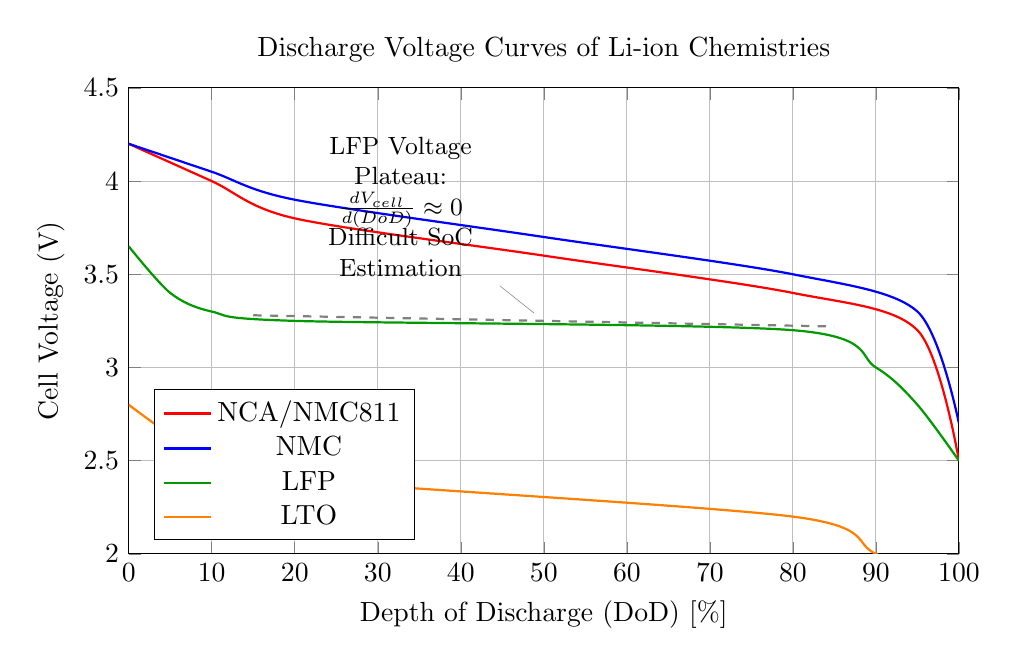
\begin{tikzpicture}
        \begin{axis}[
            title={Discharge Voltage Curves of Li-ion Chemistries},
            xlabel={Depth of Discharge (DoD) [\%]},
            ylabel={Cell Voltage (V)},
            xmin=0, xmax=100,
            ymin=2.0, ymax=4.5,
            grid=major,
            legend pos=south west,
            width=\textwidth,
            height=7.5cm,
        ]
        \addplot[smooth, thick, red] coordinates { (0, 4.2) (10, 4.0) (20, 3.8) (50, 3.6) (80, 3.4) (95, 3.2) (100, 2.5) };
        \addlegendentry{NCA/NMC811}

        \addplot[smooth, thick, blue] coordinates { (0, 4.2) (10, 4.05) (20, 3.9) (50, 3.7) (80, 3.5) (95, 3.3) (100, 2.7) };
        \addlegendentry{NMC}

        \addplot[smooth, thick, green!60!black] coordinates { (0, 3.65) (5, 3.4) (10, 3.3) (20, 3.25) (80, 3.2) (90, 3.0) (95, 2.8) (100, 2.5) };
        \addlegendentry{LFP}
        
        \addplot[smooth, thick, orange] coordinates { (0, 2.8) (10, 2.5) (20, 2.4) (80, 2.2) (90, 2.0) (100, 1.8) };
        \addlegendentry{LTO}

        \draw[dashed, thick, gray] (axis cs:15,3.28) -- (axis cs:85,3.22);
        \node[pin=135:{\parbox{2.5cm}{\centering \small LFP Voltage Plateau: \\ $\frac{dV_{cell}}{d(DoD)} \approx 0$ \\ Difficult SoC Estimation}}] at (axis cs:50,3.25) {};
        \end{axis}
    \end{tikzpicture}
    \caption{Typical discharge voltage curves for various lithium-ion chemistries. The extremely flat profile of LFP makes accurate SoC estimation challenging based on voltage alone, necessitating more complex estimation techniques like Coulomb counting and periodic recalibration.}
    \label{fig:voltage_curves_detailed}
\end{figure}
\noindent
As shown in Figure \ref{fig:voltage_curves_detailed}, LFP's remarkably flat voltage plateau makes it nearly impossible for BMS to determine precise SoC in the central operating range (from approximately 20\% to 80\%) using voltage alone. This necessitates more complex estimation techniques, such as Coulomb counting (integrating current over time), which can suffer from drift. To correct this drift, LFP-equipped vehicles require periodic full charges to 100\% for BMS recalibration. This represents an important operational constraint that V2G control strategies must consider.

\subsection{Comparative Analysis and Safety Considerations}

The trade-offs between chemistries are summarized in Table \ref{tab:chem_comparison_detailed}. Safety remains paramount, with the primary risk being thermal runaway,a dangerous, self-sustaining exothermic reaction. This risk relates directly to cathode material chemical and thermal stability. Higher energy density generally means more energy packed into smaller mass, which can be released violently if cells are compromised. Consequently, critical temperatures for initiating thermal runaway are generally lower for higher energy density chemistries. LFP's stable phosphate-based structure makes it far more resistant to thermal runaway than nickel-based counterparts, a key reason for its growing popularity.

\begin{table}[H]
\centering
\small
\caption{Comparative analysis of key automotive battery chemistries, highlighting the trade-offs between performance and safety.}
\label{tab:chem_comparison_detailed}
\begin{tabularx}{\textwidth}{
  @{}
  >{\bfseries\RaggedRight}X
  *{5}{>{\centering\arraybackslash}X}
  @{}
}
\toprule
Metric & NCA & NMC & LFP & LTO & LCO \\
\midrule
Energy Density (Wh/kg) & 200 - 260 (Highest) & 150 - 220 (High) & 90 - 160 (Moderate) & 60 - 110 (Low) & 150-200 (High) \\
\addlinespace
Cycle Life & 1000 - 2000 & 1000 - 2500 & 2000 - 5000+ & $>$10,000 & 500 - 1000 \\
\addlinespace
Safety & Good & Very Good & Excellent & Excellent & Poor \\
\addlinespace
Thermal Runaway Temp ($^{\circ}$C) & $\sim$150 - 180 & $\sim$180 - 210 & $\sim$220 - 270 & $>$ 250 & $\sim$150 \\
\bottomrule
\end{tabularx}
\end{table}